\chapter{TINJAUAN PUSTAKA}

Bab Studi Literatur digunakan untuk mendeskripsikan kajian literatur yang terkait dengan persoalan tugas akhir. Tujuan studi literatur adalah:

\begin{enumerate}
	\item menunjukkan kepada pembaca adanya gap seperti pada rumusan masalah yang memang belum terselesaikan,
	\item memberikan pemahaman yang secukupnya kepada pembaca tentang teori atau pekerjaan terkait yang terkait langsung dengan penyelesaian persoalan, serta
	\item menyampaikan informasi apa saja yang sudah ditulis/dilaporkan oleh pihak lain (peneliti/Tugas Akhir/Tesis) tentang hasil penelitian/pekerjaan mereka yang sama atau mirip kaitannya dengan persoalan tugas akhir.
\end{enumerate}

\section{Dasar Teori}
Perujukan literatur dapat dilakukan dengan menambahkan entri baru di berkas \texttt{references.bib}. Ada dua cara untuk melakukan perujukan dalam teks utama: perujukan di akhir kalimat dan perujukan langsung. Perujukan di akhir kalimat dilakukan menggunakan perintah \texttt{\textbackslash parencite} seperti ini \parencite{knuth:2001:art}. Sedangkan menurut \textcite{vogels:2006:web} perujukan langsung di dalam kalimat seperti ini dilakukan dengan perintah \texttt{\textbackslash textcite}.

\section{Bekerja dengan Float}

Float adalah \textit{container} untuk elemen-elemen dokumen yang tidak dapat dipisah menjadi beberapa halaman. Environment ``table'' dan ``figure'' secara default adalah float. Float berguna untuk memudahkan peletakan objek yang tidak cukup jika diletakkan di halaman sekarang. Peletakan float diatur oleh \LaTeX\ dan pengguna sebaiknya memberikan keleluasaan kepada \LaTeX\ agar dapat mengatur peletakan dengan baik.

\subsection{Gambar}

Float bisa di-\textit{cross reference}. Contohnya Gambar~\ref{fig:contoh_gambar} adalah contoh gambar.

\begin{figure}[h]
	\centering
	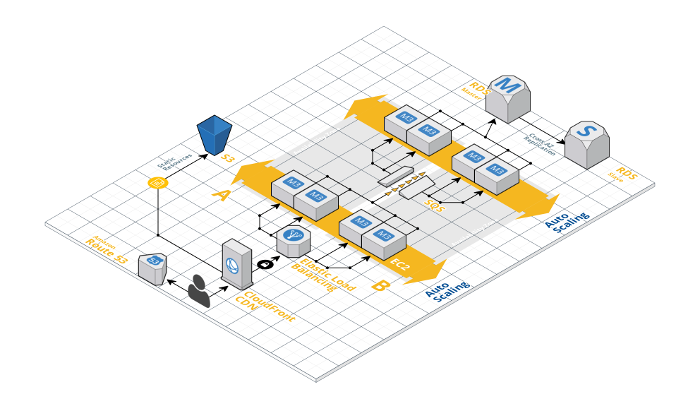
\includegraphics[width=\textwidth]{assets/chapter-2-infrastructure-diagram.png}
	\caption{Contoh gambar}
	\label{fig:contoh_gambar}
\end{figure}

\subsection{Tabel}

Tabel juga merupakan float. Tabel~\ref{table:contoh_tabel} adalah contoh tabel. Perhatikan bahwa walaupun didefinisikan setelah paragraf ini, tabel tidak diletakkan tepat di bawah paragraf ini pada dokumen hasil kompilasi. Hal ini karena ukuran (tinggi) tabel tidak cukup apabila diletakkan di sisa halaman ini. \LaTeX-lah yang mengatur peletakan tabel. Oleh karena itu tidak disarankan untuk merujuk tabel (dan objek float lain) dengan frasa ``Tabel di bawah ini'', ``Tabel berikut'', dan sebagainya.

\begin{table}[htbp]
	\centering
	\caption{Contoh Tabel}
	\label{table:contoh_tabel}
	\begin{tabular}{ll}
		\toprule
		\multicolumn{1}{l}{\textbf{Contoh Judul Kolom}} & \multicolumn{1}{l}{\textbf{Nilai}} \\
		\midrule
		Besaran 1                                       & 12 meter                           \\
		Besaran 2                                       & $360^\circ$                        \\
		Besaran 3                                       & 0,2 meter                          \\
		Besaran 4                                       & $1^\circ$                          \\
		Besaran 5                                       & 8000 sampel/detik                  \\
		\bottomrule
	\end{tabular}
\end{table}

\section{Persamaan Matematika}

Persamaan~\eqref{eq:contoh_equation} adalah contoh persamaan matematika,

\begin{align}
	c^2 = a^2 + b^2\,.
	\label{eq:contoh_equation}
\end{align}

Contoh penggunaan notasi custom,

\begin{align}
	\bayes{x}{y}\,.
	\label{eq:contoh_equation_custom}
\end{align}

\section{Menulis Algoritma dan Pseudocode}

Blok algoritma dan \textit{pseudocode} secara teknis juga merupakan sebuah float. Untuk dapat menggunakan algoritma ada beberapa \textit{package} yang perlu di-\textit{import} (sudah ter-\textit{import} di dokumen ini): \texttt{algorithm} dan \texttt{algpseudocode}. Algoritma \ref{alg:example} adalah contoh blok algoritma.

\begin{algorithm}
	\begin{algorithmic}[1]
		\Function{Example\_algorithm}{$a,b,c$}
		\State $p \gets [~]$
		\For {$a_i \in a$}
		\If{$a_i > 0$}
		\State $p_i \gets a_i + b$
		\Else
		\State $p_i \gets a_i - c$
		\EndIf
		\EndFor
		\State \Return $p$
		\EndFunction
	\end{algorithmic}
	\caption{Contoh Algoritma}
	\label{alg:example}
\end{algorithm}

\section{Studi Terkait}
\blindtext
